% GNUPLOT: LaTeX picture with Postscript
\begingroup
  \makeatletter
  \providecommand\color[2][]{%
    \GenericError{(gnuplot) \space\space\space\@spaces}{%
      Package color not loaded in conjunction with
      terminal option `colourtext'%
    }{See the gnuplot documentation for explanation.%
    }{Either use 'blacktext' in gnuplot or load the package
      color.sty in LaTeX.}%
    \renewcommand\color[2][]{}%
  }%
  \providecommand\includegraphics[2][]{%
    \GenericError{(gnuplot) \space\space\space\@spaces}{%
      Package graphicx or graphics not loaded%
    }{See the gnuplot documentation for explanation.%
    }{The gnuplot epslatex terminal needs graphicx.sty or graphics.sty.}%
    \renewcommand\includegraphics[2][]{}%
  }%
  \providecommand\rotatebox[2]{#2}%
  \@ifundefined{ifGPcolor}{%
    \newif\ifGPcolor
    \GPcolortrue
  }{}%
  \@ifundefined{ifGPblacktext}{%
    \newif\ifGPblacktext
    \GPblacktexttrue
  }{}%
  % define a \g@addto@macro without @ in the name:
  \let\gplgaddtomacro\g@addto@macro
  % define empty templates for all commands taking text:
  \gdef\gplbacktext{}%
  \gdef\gplfronttext{}%
  \makeatother
  \ifGPblacktext
    % no textcolor at all
    \def\colorrgb#1{}%
    \def\colorgray#1{}%
  \else
    % gray or color?
    \ifGPcolor
      \def\colorrgb#1{\color[rgb]{#1}}%
      \def\colorgray#1{\color[gray]{#1}}%
      \expandafter\def\csname LTw\endcsname{\color{white}}%
      \expandafter\def\csname LTb\endcsname{\color{black}}%
      \expandafter\def\csname LTa\endcsname{\color{black}}%
      \expandafter\def\csname LT0\endcsname{\color[rgb]{1,0,0}}%
      \expandafter\def\csname LT1\endcsname{\color[rgb]{0,1,0}}%
      \expandafter\def\csname LT2\endcsname{\color[rgb]{0,0,1}}%
      \expandafter\def\csname LT3\endcsname{\color[rgb]{1,0,1}}%
      \expandafter\def\csname LT4\endcsname{\color[rgb]{0,1,1}}%
      \expandafter\def\csname LT5\endcsname{\color[rgb]{1,1,0}}%
      \expandafter\def\csname LT6\endcsname{\color[rgb]{0,0,0}}%
      \expandafter\def\csname LT7\endcsname{\color[rgb]{1,0.3,0}}%
      \expandafter\def\csname LT8\endcsname{\color[rgb]{0.5,0.5,0.5}}%
    \else
      % gray
      \def\colorrgb#1{\color{black}}%
      \def\colorgray#1{\color[gray]{#1}}%
      \expandafter\def\csname LTw\endcsname{\color{white}}%
      \expandafter\def\csname LTb\endcsname{\color{black}}%
      \expandafter\def\csname LTa\endcsname{\color{black}}%
      \expandafter\def\csname LT0\endcsname{\color{black}}%
      \expandafter\def\csname LT1\endcsname{\color{black}}%
      \expandafter\def\csname LT2\endcsname{\color{black}}%
      \expandafter\def\csname LT3\endcsname{\color{black}}%
      \expandafter\def\csname LT4\endcsname{\color{black}}%
      \expandafter\def\csname LT5\endcsname{\color{black}}%
      \expandafter\def\csname LT6\endcsname{\color{black}}%
      \expandafter\def\csname LT7\endcsname{\color{black}}%
      \expandafter\def\csname LT8\endcsname{\color{black}}%
    \fi
  \fi
    \setlength{\unitlength}{0.0500bp}%
    \ifx\gptboxheight\undefined%
      \newlength{\gptboxheight}%
      \newlength{\gptboxwidth}%
      \newsavebox{\gptboxtext}%
    \fi%
    \setlength{\fboxrule}{0.5pt}%
    \setlength{\fboxsep}{1pt}%
\begin{picture}(9340.00,5660.00)%
    \gplgaddtomacro\gplbacktext{%
      \colorrgb{0.00,0.00,0.00}%%
      \put(1018,787){\makebox(0,0)[r]{\strut{} 0,000}}%
      \colorrgb{0.00,0.00,0.00}%%
      \put(1018,1252){\makebox(0,0)[r]{\strut{} 0,005}}%
      \colorrgb{0.00,0.00,0.00}%%
      \put(1018,1718){\makebox(0,0)[r]{\strut{} 0,010}}%
      \colorrgb{0.00,0.00,0.00}%%
      \put(1018,2183){\makebox(0,0)[r]{\strut{} 0,015}}%
      \colorrgb{0.00,0.00,0.00}%%
      \put(1018,2648){\makebox(0,0)[r]{\strut{} 0,020}}%
      \colorrgb{0.00,0.00,0.00}%%
      \put(1018,3114){\makebox(0,0)[r]{\strut{} 0,025}}%
      \colorrgb{0.00,0.00,0.00}%%
      \put(1018,3579){\makebox(0,0)[r]{\strut{} 0,030}}%
      \colorrgb{0.00,0.00,0.00}%%
      \put(1018,4044){\makebox(0,0)[r]{\strut{} 0,035}}%
      \colorrgb{0.00,0.00,0.00}%%
      \put(1018,4509){\makebox(0,0)[r]{\strut{} 0,040}}%
      \colorrgb{0.00,0.00,0.00}%%
      \put(1018,4975){\makebox(0,0)[r]{\strut{} 0,045}}%
      \colorrgb{0.00,0.00,0.00}%%
      \put(1018,5440){\makebox(0,0)[r]{\strut{} 0,050}}%
      \colorrgb{0.00,0.00,0.00}%%
      \put(1202,481){\makebox(0,0){\strut{} 0,0}}%
      \colorrgb{0.00,0.00,0.00}%%
      \put(1908,481){\makebox(0,0){\strut{} 0,1}}%
      \colorrgb{0.00,0.00,0.00}%%
      \put(2613,481){\makebox(0,0){\strut{} 0,2}}%
      \colorrgb{0.00,0.00,0.00}%%
      \put(3319,481){\makebox(0,0){\strut{} 0,3}}%
      \colorrgb{0.00,0.00,0.00}%%
      \put(4024,481){\makebox(0,0){\strut{} 0,4}}%
      \colorrgb{0.00,0.00,0.00}%%
      \put(4730,481){\makebox(0,0){\strut{} 0,5}}%
      \colorrgb{0.00,0.00,0.00}%%
      \put(5435,481){\makebox(0,0){\strut{} 0,6}}%
      \colorrgb{0.00,0.00,0.00}%%
      \put(6141,481){\makebox(0,0){\strut{} 0,7}}%
      \colorrgb{0.00,0.00,0.00}%%
      \put(6846,481){\makebox(0,0){\strut{} 0,8}}%
      \colorrgb{0.00,0.00,0.00}%%
      \put(7551,481){\makebox(0,0){\strut{} 0,9}}%
      \colorrgb{0.00,0.00,0.00}%%
      \put(8257,481){\makebox(0,0){\strut{} 1,0}}%
      \colorrgb{0.00,0.00,0.00}%%
      \put(8441,787){\makebox(0,0)[l]{\strut{} 0}}%
      \colorrgb{0.00,0.00,0.00}%%
      \put(8441,1252){\makebox(0,0)[l]{\strut{} 2}}%
      \colorrgb{0.00,0.00,0.00}%%
      \put(8441,1718){\makebox(0,0)[l]{\strut{} 4}}%
      \colorrgb{0.00,0.00,0.00}%%
      \put(8441,2183){\makebox(0,0)[l]{\strut{} 6}}%
      \colorrgb{0.00,0.00,0.00}%%
      \put(8441,2648){\makebox(0,0)[l]{\strut{} 8}}%
      \colorrgb{0.00,0.00,0.00}%%
      \put(8441,3114){\makebox(0,0)[l]{\strut{} 10}}%
      \colorrgb{0.00,0.00,0.00}%%
      \put(8441,3579){\makebox(0,0)[l]{\strut{} 12}}%
      \colorrgb{0.00,0.00,0.00}%%
      \put(8441,4044){\makebox(0,0)[l]{\strut{} 14}}%
      \colorrgb{0.00,0.00,0.00}%%
      \put(8441,4509){\makebox(0,0)[l]{\strut{} 16}}%
      \colorrgb{0.00,0.00,0.00}%%
      \put(8441,4975){\makebox(0,0)[l]{\strut{} 18}}%
      \colorrgb{0.00,0.00,0.00}%%
      \put(8441,5440){\makebox(0,0)[l]{\strut{} 20}}%
    }%
    \gplgaddtomacro\gplfronttext{%
      \csname LTb\endcsname%%
      \put(291,3113){\makebox(0,0){\strut{}$s$}}%
      \csname LTb\endcsname%%
      \put(8938,3113){\rotatebox{-270}{\makebox(0,0){\strut{}$I_1\, / \,\unit{A}$}}}%
      \csname LTb\endcsname%%
      \put(4729,153){\makebox(0,0){\strut{}$P\ped{m}/P\ped{m,n}$}}%
      \csname LTb\endcsname%%
      \put(4729,5331){\makebox(0,0){\strut{}}}%
      \csname LTb\endcsname%%
      \put(4729,5440){\makebox(0,0){\strut{}}}%
      \csname LTb\endcsname%%
      \put(7801,1530){\makebox(0,0){\strut{}}}%
      \csname LTb\endcsname%%
      \put(7918,1448){\makebox(0,0)[l]{\strut{}$s$}}%
      \csname LTb\endcsname%%
      \put(7918,1120){\makebox(0,0)[l]{\strut{}$I_1$}}%
      \csname LTb\endcsname%%
      \put(4624,1485){\rotatebox{-270}{\makebox(0,0){$\scriptstyle\num{0.5}$}}}%
      \csname LTb\endcsname%%
      \put(7199,3207){\makebox(0,0){$\scriptstyle\qty{9,7}{A}$}}%
      \csname LTb\endcsname%%
      \put(2260,2974){\makebox(0,0){$\scriptstyle\num{0,0226}$}}%
    }%
    \gplbacktext
    \put(0,0){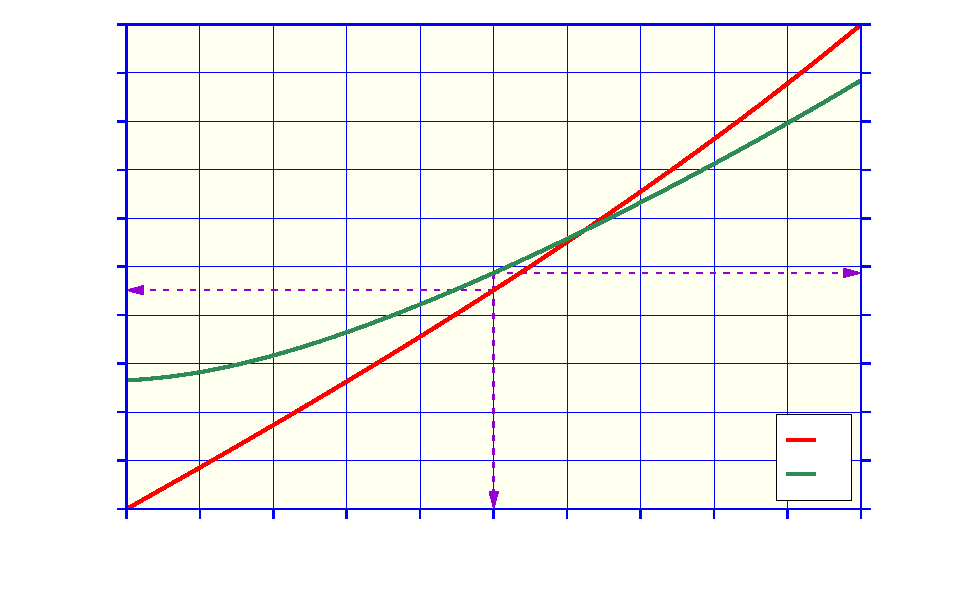
\includegraphics{Cap-Motors-Induccio-MotCarregaReduida-1}}%
    \gplfronttext
  \end{picture}%
\endgroup
